\chapter{Distributed Memory Systems}

The first issue to address is the communication between different nodes. The main problem is that the memory is distributed, so we need to find a way to communicate between different nodes.

\section{Interconnection Networks}
Interconnection networks for parallel systems share many technical features of WAN, but they have very different requirements:
\begin{itemize}
   \item $\mathcal{O}(10^1 \div 10^5)$ nodes
   \item Distances ranging in $\mathcal{O}(10^0 \div 10^1)$ meters
\end{itemize}

Key metrics for us are:
\begin{itemize}
   \item \textbf{Latency} - time lapse between the instant a packet starts to be transmitted and the instant it is ---entirely--- received
   \begin{itemize}
      \item \textbf{No-load} (or \textit{Zero-load}) latency: the latency experienced by a packet when there is no other traffic on the network
      \item \textbf{Under-load} latency: the latency experienced by a packet when there is other traffic on the network, but \ul{below the \textit{saturation point}}
      \note{\textit{Saturation point} is a crucial threshold we will discuss in future.}
   \end{itemize}
   \item (Offered) \textbf{Throughput} - the amount of data that transmitted over the network in a given time.
   The \textbf{Saturation Throughput} is the maximum amount of traffic sustained by the network, it is the point at which the network is fully loaded. 
   \item \textbf{Bandwidth} - theoretical maximum data transfer rate under ideal conditions on a network path.
\end{itemize}

\note{Two aspects which are fundamental but which we won't address are:
\begin{itemize}
   \item \textbf{Routing}
   \item \textbf{Flow control}
\end{itemize}}

\subsection{Terminology}

\note{Endpoints, links, switches\dots}

\begin{itemize}
   \item \textbf{Direct Network} aka \textit{static} - nodes are both endpoints and switches
   \item \textbf{Indirect Network} aka \textit{dynamic} - endpoints are connected indirectly through switches
\end{itemize}

\begin{itemize}
   \item \textbf{Degree} - number of maximum neighbors a node can have
   \item \textbf{Diameter} - longest of shortest paths between any two nodes
   \note{maximum (minimum) distance between two nodes}
   \item \textbf{Bisection width} - minimum number of links that must be removed to split the network into two equal halves
\end{itemize}

\subsection{Examples}
\begin{figure}[htbp]
   \centering
   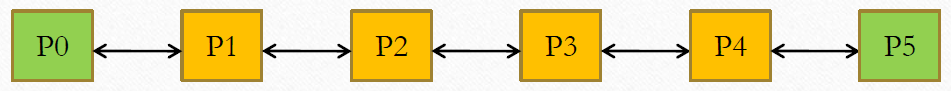
\includegraphics{images/05/linear_array.png}
   \caption{Linear Array topology}
   \label{fig:05/linear_array}

   $degree = 2 \quad Diameter = n-1 \quad bw = 1$
\end{figure}

\begin{figure}[htbp]
   \centering
   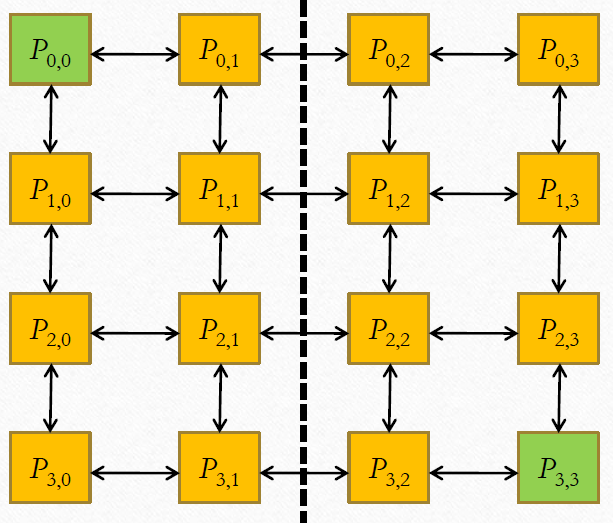
\includegraphics{images/05/2d_mesh.png}
   \caption{2D Mesh topology}
   \label{fig:05/2d_mesh}
   $M(d,d)$ has $n=d^2$ endpoints
   $degree = 4 \quad Diameter = 2(d-1) = \mathcal{O}(\sqrt{n}) \quad bw = d = \mathcal{O}(\sqrt{n})$
\end{figure}

\begin{figure}[htbp]
   \centering
   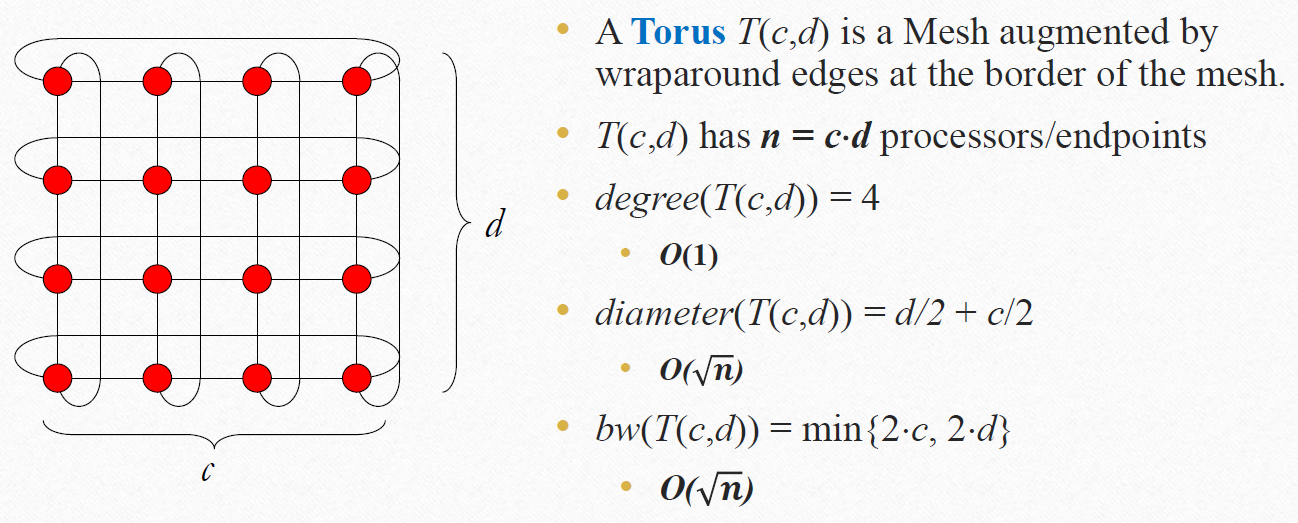
\includegraphics{images/05/torus.png}
   \caption{Torus topology}
   \label{fig:05/torus}
\end{figure}

\begin{figure}[htbp]
   \centering
   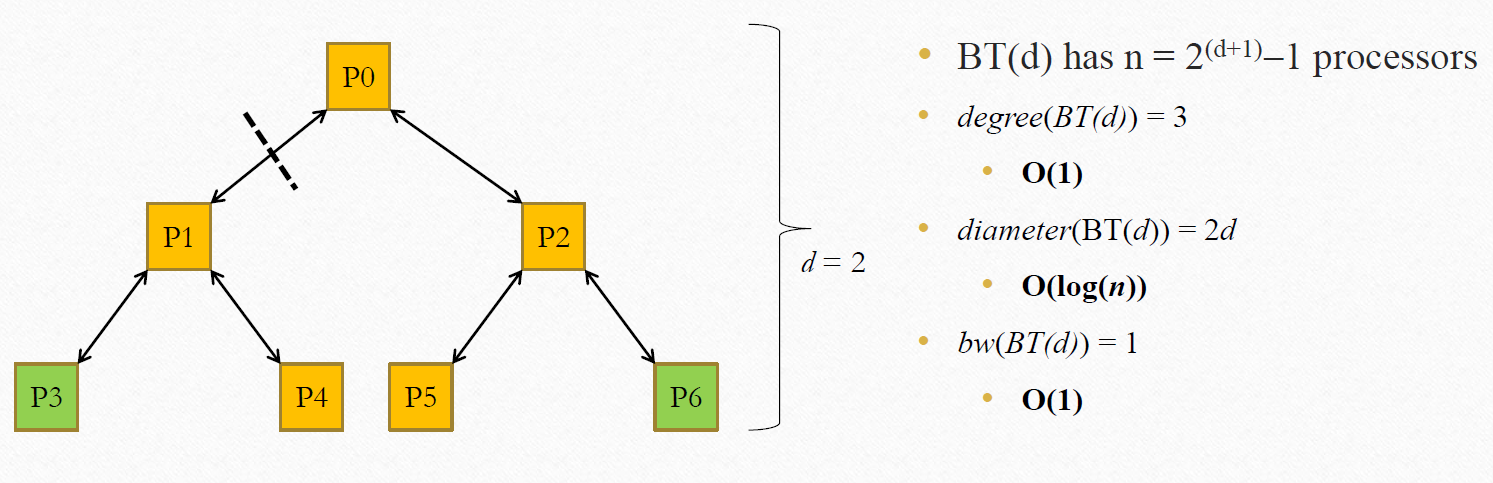
\includegraphics{images/05/bintree.png}
   \caption{Binary Tree topology}
   \label{fig:05/bintree}
\end{figure}

\subsubsection{Hypercube}
\begin{figure}[htbp]
   \centering
   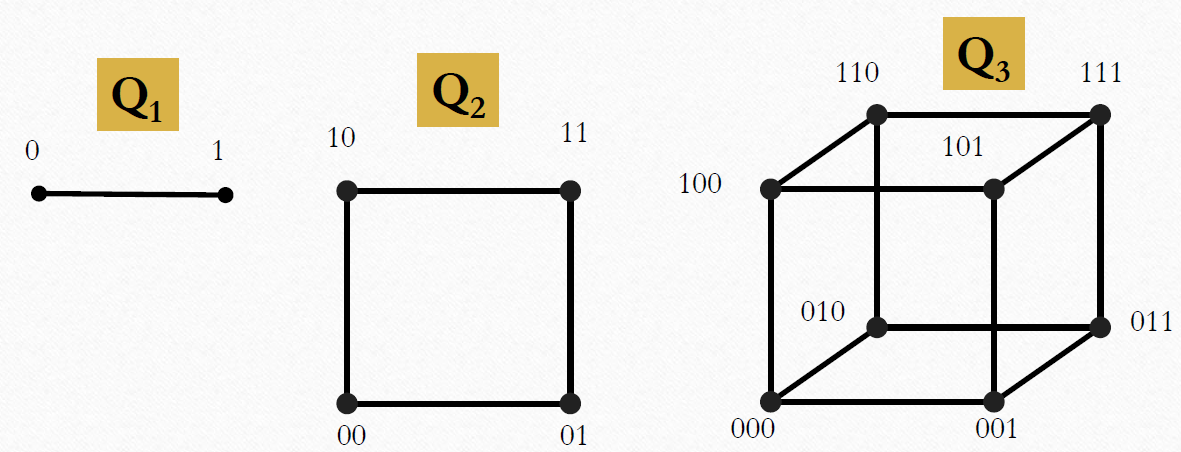
\includegraphics{images/05/hypercube1.png}
   \caption{Hypercube topology}
   \label{fig:05/hypercube1}
\end{figure}

The hypercube $\mathcal{Q}_d(d\geq1)$ is the graph that has vertices representing the $2^d$ binary strings of length $d$. Two vertices are adjacent if their binary strings differ in \textit{exactly} one bit.

The hypercube is a very interesting topology because it has a very low diameter and bisection width, but it is very expensive to build.

\subsection{Criteria for Evaluation - Summary}
So, what do we want from an interconnection network?

\begin{itemize}
   \item \textit{Constant} \textbf{degree} - Allows scaling the network without increasing the degree of the nodes
   \item \textit{Low} \textbf{Diameter} - Allows for low latency
   \item \textit{High} \textbf{bisection width} - Allows for high bandwidth, but may require to have dynamic degree.
\end{itemize}

\subsubsection{Simple Communication cost model}
\begin{equation}\label{eq:05/comm_cost_model}
   T_{comm} = t_0 + n \times s \approx \begin{cases}
      t_0 & \textit{for small n}\\
      n \times s & \textit{for large n}
   \end{cases}
\end{equation}

\begin{itemize}
   \item $t_0$ start-up time (network and communication runtime setup)
   \begin{itemize}
      \item Includes all costs for sending the shortest message. (\textit{latency})
      \item Its value may be different for different programming models
   \end{itemize}
   \item $n$ amount of (e.g. bytes) data to be transferred
   \item $s$ transmission cost. Usually $s = \frac{1}{B}$ with $B$ available bandwidth on the path
   \begin{itemize}
      \item $s$ il limited by the slowest part of the path between the sender and the receiver processes
      \item $s$ includes both SW agents (e.g. app max output rate) and HW agents (e.g. network max throughput)
   \end{itemize}
\end{itemize}

\subsection{More advanced topologies}
\begin{itemize}
   \item \textbf{Fat-tree} - a tree-like topology that has a high bisection width
   \item \textbf{Dragonfly} - a topology that combines a tree-like structure with a mesh-like structure
   \item \textbf{Jellyfish} - a topology that is based on a random graph
\end{itemize}

\newpage
\subsubsection{Fat-tree}
\begin{paracol}{2}
   
   All leaves are endpoints and all internal nodes are switches.
   Links higher in the tree have higher bandwidth.
   The idea is to keep the bandwidth constant across the tree.

   The key issue is the cost, which increases with the depth of the tree.
   To overcome this problem, we can use a \textbf{Spine-Leaf} topology, where the tree is split into two parts: the spine and the leaves.
   \note{In the slides this is considered as a different implementation of the fat-tree, but it is actually a different topology.}

   \switchcolumn
   \begin{figure}[htbp]
      \centering
      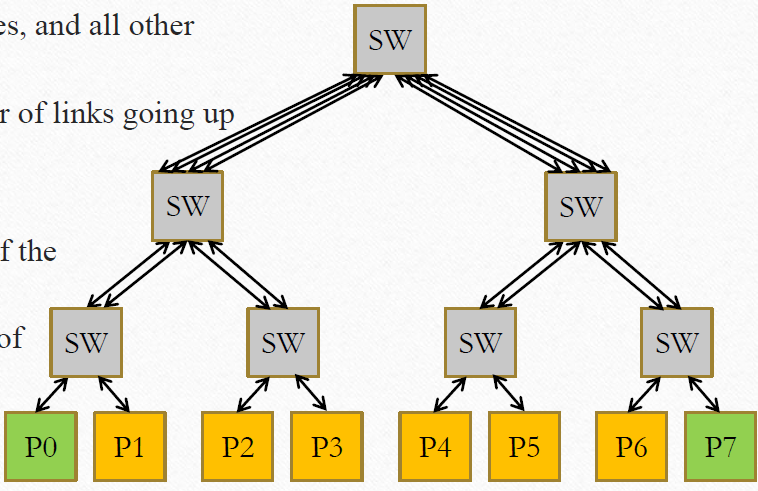
\includegraphics{images/05/fat_tree.png}
      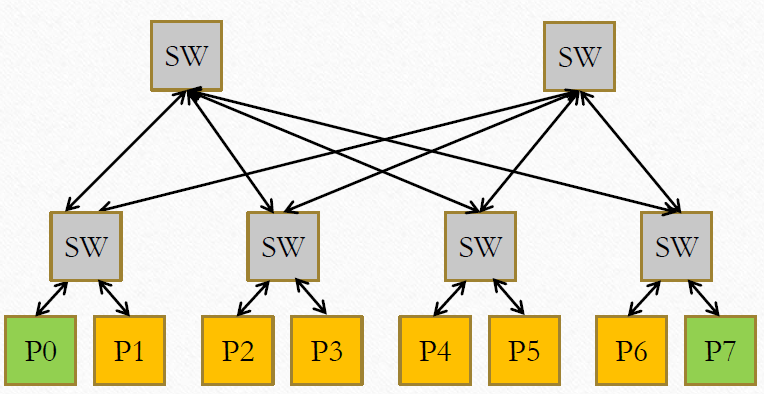
\includegraphics{images/05/fat_tree2.png}
      \caption{Fat tree and Spine Leaf}
      \label{fig:05/fat_tree}
   \end{figure}
   
\end{paracol}

\subsubsection{Dragonfly}

\begin{paracol}{2}
   
   This is the most used network used in supercomputers. It is divided in three levels:
   \begin{enumerate}
      \item Router
      \item Group
      \item System
   \end{enumerate}
   
   Each router has connections to $p$ endpoints, $a-1$ local channels (to other routers in the same group) and $h$ global channels (to routers in other groups).
   
   A group consists of $a$ routers and group has $ap$ connections to endpoints, and $ah$ connections to other groups.
   
   \switchcolumn
   \begin{figure}[htbp]
      \centering
      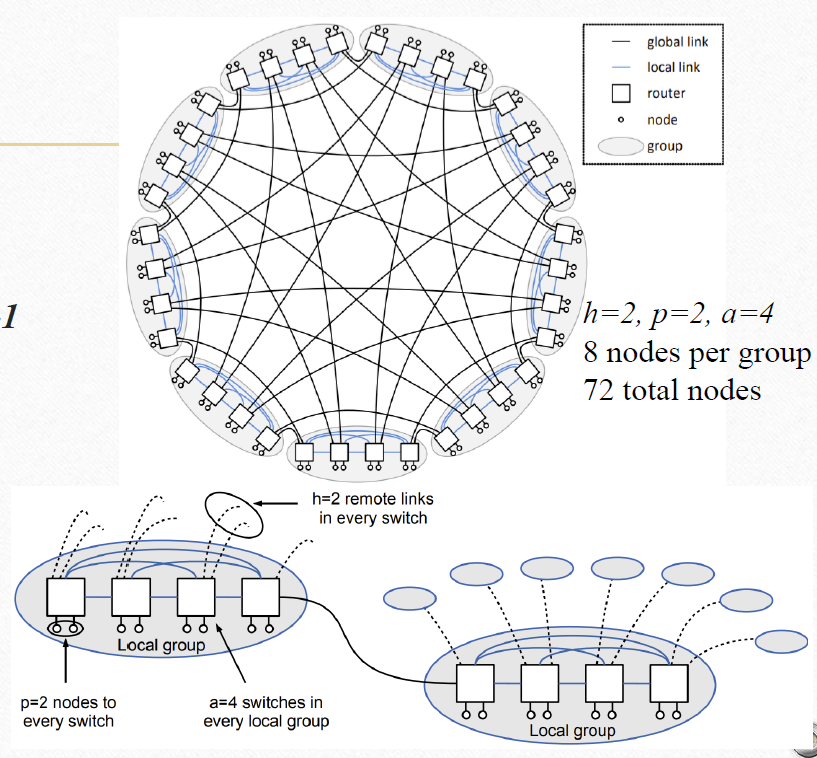
\includegraphics{images/05/dragonfly.png}
      \caption{Dragonfly}
      \label{fig:05/dragonfly}
   \end{figure}
\end{paracol}

\section{Computation-to-Communication Overlap}

It is always udeful for the sender to execute a \textbf{non-blocking send} to the destination process: the NICE executes the data transfer in the background, and then notifies the sender process when the tranmission is completed, so that the sender can continue with its computation.
This creates a partial or full \textit{overlap} between computation and communication.

\textit{How can we achieve this overlap?}

\subsection{Syncronous vs Asynchronous Communication}

The \textbf{asynchrony degree} of a channel is the maximum number of messages that can be sent on the channel without waiting for the receiver to start receiving data.
Essentially, it is the length of the queue of messages that can be sent on the channel.

\begin{itemize}
   \item \textbf{Synchronous} - the operation comples only after the message has been received/sent. i.e. a peer \textbf{blocks} until the other peer completes the operation.
   \item \textbf{Asynchronous} - the communication operation returns immediately, without waiting for the message to be effectively sent/received.
   \begin{itemize}
      \item The completion/success will be tested later on
      \item The number of messages that can be sent depends on the \textbf{asynchrony degree} of the channel.
   \end{itemize}
\end{itemize}

Note also that sometimes \textbf{input non-determinism} must be taken into account:
the \textit{receive} operation may return a message from any channels in the set, and the message picking algorithm is random and non-predictable.

\begin{figure}[htbp]
   \centering
   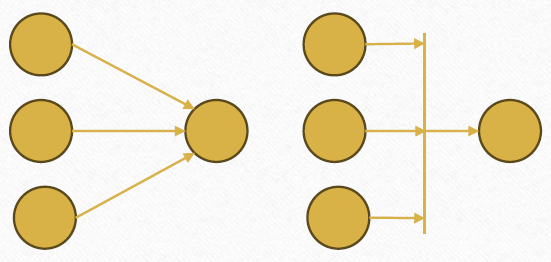
\includegraphics{images/05/input_determism.png}
   \caption{Input non-determinism}
   \label{fig:05/input_determism}
\end{figure}

\section{Foster's Parallel Algorithm Design Method}
There is no one-fits-all recipe for parallelizing sequential programs, however\dots Foster's \textbf{PCAM} approach provides some useful guidelines to keep in mind when designing parallel algorithms.

\begin{itemize}
   \item \textbf{Partitioning} - divide the problem into a large amount of small fine-grained tasksk that can be executed in parallel
   \item \textbf{Communication} - determine the required communication pattern between the tasks (\textit{data dependencies})
   \item \textbf{Aggolmeration} - combine identified tasks into larger coarse-grained tasks to \ul{reduce communication by improving data locality}
   \item \textbf{Mapping} - assign tasks to processes and threads to minimize communication, enable concurrency and \textit{balance workload}
\end{itemize}

\subsection{Jacobi and MCOP}

In Lecture 7, more concepts concerning Jacobi and Matrix Chain Ordering Problem (MCOP) are be discussed.
They are not reported here.

\begin{figure}[htbp]
   \centering
   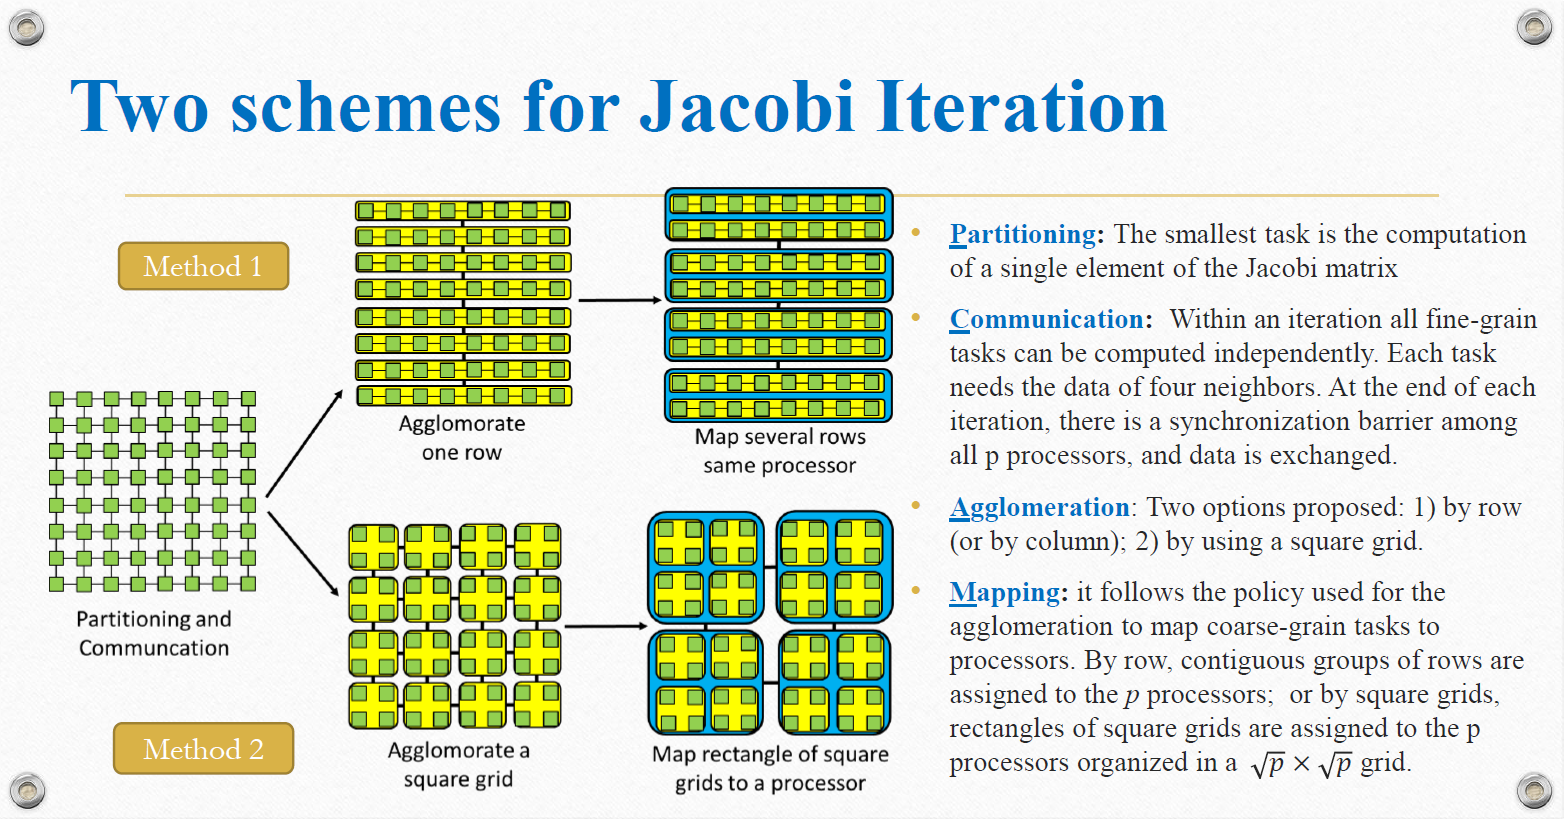
\includegraphics{images/05/jacobi.png}
   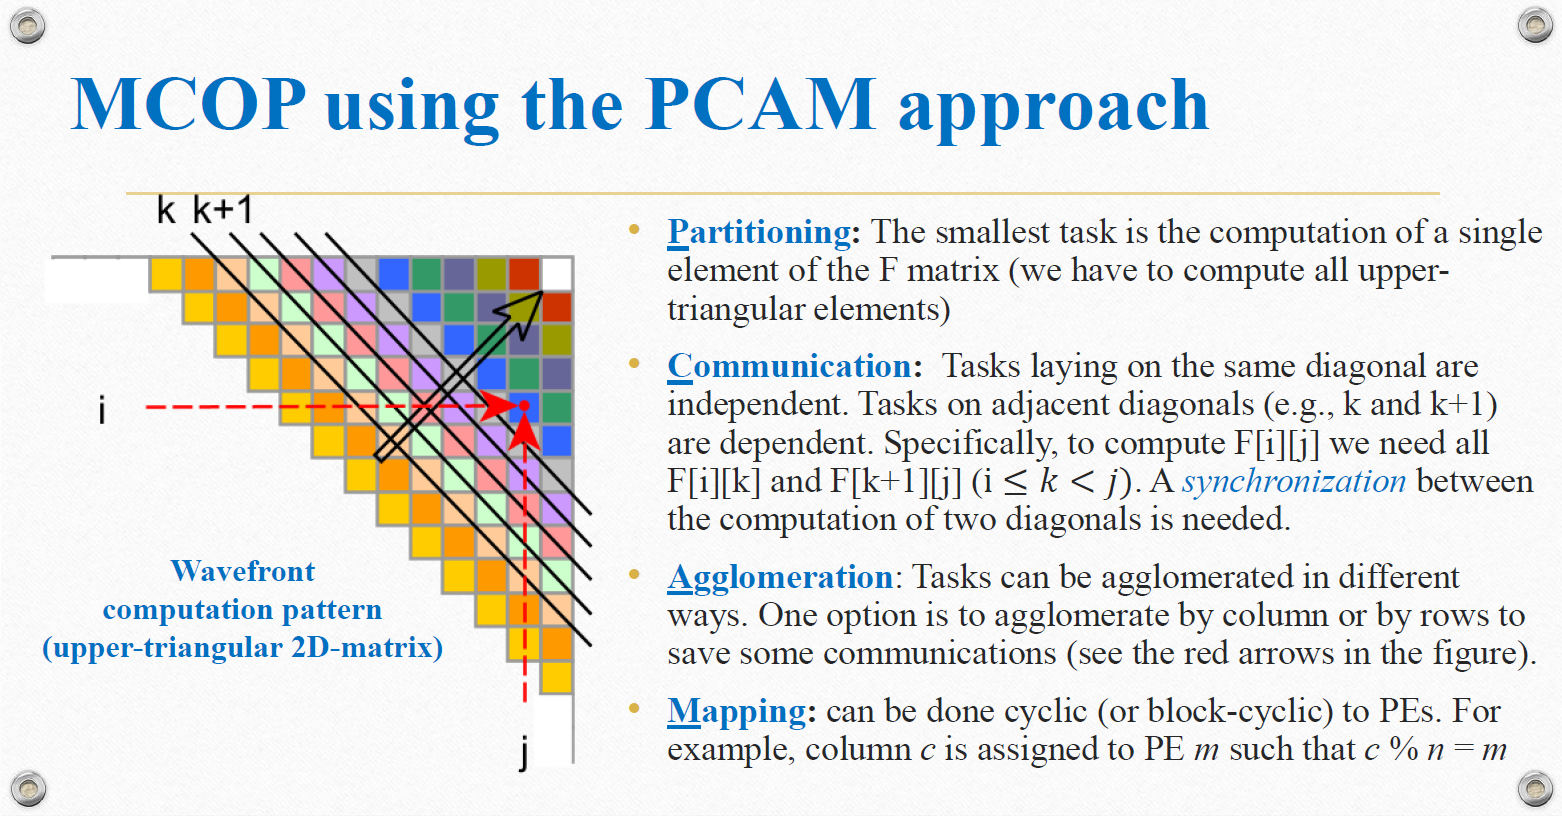
\includegraphics{images/05/mcop.png}
   \caption{Jacobi and MCOP slides}
   \label{fig:05/jacobi_mcop}
\end{figure}